\documentclass[a4paper]{article}
\usepackage{graphicx}  
\usepackage[landscape]{geometry}
%\usepackage[pdftex]{color}
\usepackage[dvipdfm]{color}
%\usepackage{url}
\usepackage{quickrefcard}


\usepackage{multicol}
\usepackage{amsmath}
\usepackage{amsfonts}

\pagestyle{empty}
\newcommand{\kr}[2]{\left(\frac{#1}{#2}\right)}

%\newcommand{\ZZ}{\mathbf{Z}}
%\newcommand{\FF}{\mathbf{F}}
%\newcommand{\QQ}{\mathbf{Q}}

\newcommand{\ZZ}{\mathbb{Z}}
\newcommand{\FF}{\mathbb{F}}
\newcommand{\QQ}{\mathbb{Q}}

\begin{document}
\begin{multicols*}{3}
\begin{center}
\textbf{Sage Quick Reference:\\Elementary Number Theory}\\
William Stein (modified by nu)\\
Sage Version 3.4\\
\url{http://wiki.sagemath.org/quickref}\\
GNU Free Document License, extend for your own use\\
\end{center}
\vspace{-2ex}

\sect{}
Everywhere $m,n,a,b, etc.$ are elements of \EX{ZZ}
\BreakLineAndIndent
\sagecommand{ZZ} $=\ZZ = $ all integers 
%*********************************************

\sect{Integers}
\vspace{-2ex}
$$\ldots, -2, -1, 0, 1, 2, 3, 4, 5, 6, 7, 8, 9, 10, \ldots$$
\vspace{-4ex}

$n$ divided by $m$ has {\em remainder} {\ex \verb|n % m|}

\EX{gcd(n,m)}, \EX{gcd(}\EXVAR{list}\EX{)}

extended gcd $g = sa + tb=\gcd(a,b)$: \EX{g,s,t=xgcd(a,b)}

\EX{lcm(n,m)}, \EX{lcm(}\EXVAR{list}\EX{)}

binomial coefficient $\binom{m}{n} = $ \EX{binomial(m,n)}

digits in a given base: \EX{n.digits(}\EXVAR{base}\EX{)}

number of digits: \EX{n.ndigits(}\EXVAR{base}\EX{)}

(\sagevar{base} is optional and defaults to $10$)

divides $n\mid m$: \EX{n.divides(m)} if $nk=m$ some $k$

divisors -- all $d$ with $d\mid n$: \EX{n.divisors()}

factorial -- $n! = $ \EX{n.factorial()}


%*********************************************
\sect{Prime Numbers}
\vspace{-1ex}
$$2, 3, 5, 7, 11, 13, 17, 19, 23, 29, 31, 37, 41, 43, 47, \ldots$$
\vspace{-4ex}

factorization: \EX{factor(n)}

primality testing: \EX{is_prime(n)}, \EX{is_pseudoprime(n)}

prime power testing: \EX{is_prime_power(n)}

$\pi(x) = \#\{p: p \leq x\text{ is prime}\} = $ \EX{prime_pi(x)}

set of prime numbers: \EX{Primes()}

$\{p : m \leq p < n\text{ and $p$ prime}\} = $\EX{prime_range(m,n)}

prime powers: \EX{prime_powers(m,n)} 

first $n$ primes: \EX{primes_first_n(n)}

next and previous primes: 
\EX{next_prime(n)},          \BreakLineAndIndent
\EX{previous_prime(n)},  
\EX{next_probable_prime(n)}

prime powers:
\EX{next_prime_power(n)},    \BreakLineAndIndent
\EX{pevious_prime_power(n)}


Lucas-Lehmer test for primality of $2^p-1$
{                                             \ex\BreakLineAndIndent
\verb|def is_prime_lucas_lehmer(p):|           \BreakLineAndIndent
\verb|    s = Mod(4, 2^p - 1)|                 \BreakLineAndIndent
\verb|    for i in range(3, p+1): s = s^2 - 2| \BreakLineAndIndent
\verb|    return s == 0|}



%*********************************************
\sect{Modular Arithmetic and Congruences}

{\tiny
\verb|k=12; m = matrix(ZZ, k, [(i*j)%k for i in [0..k-1] for j in [0..k-1]]); m.plot(cmap='gray')|}
\BreakLineAndIndent
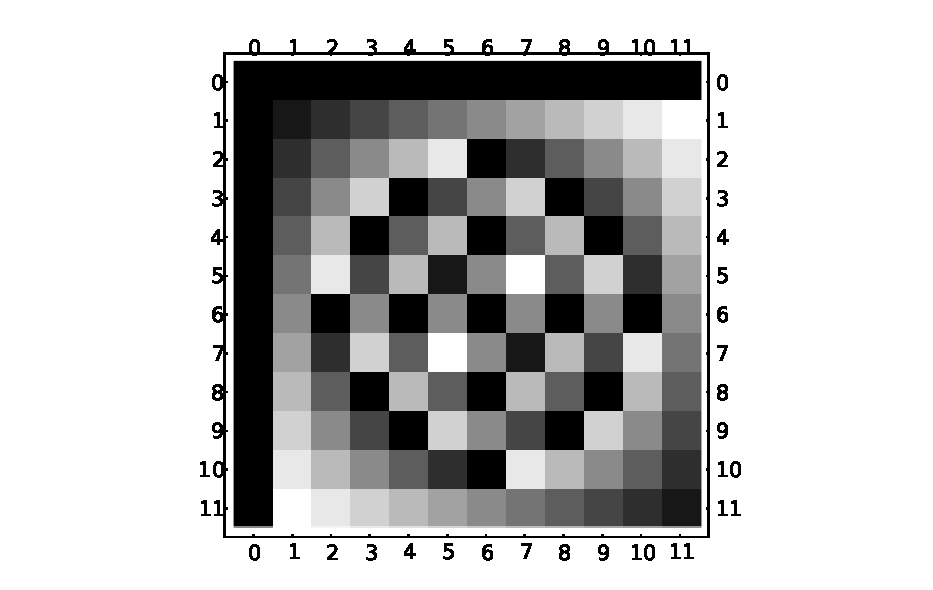
\includegraphics[width=14em]{mod12.eps}

Euler's $\phi(n)$ function: \EX{euler_phi(n)}

Kronecker symbol $\kr{a}{b} = $ \EX{kronecker_symbol(a,b)}

Quadratic residues: \EX{quadratic_residues(n)}

Quadratic non-residues: \EX{quadratic_residues(n)}

ring $\ZZ/n\ZZ = $ \EX{Zmod(n) = IntegerModRing(n)}

$a$ modulo $n$ as element of $\ZZ/n\ZZ$: \EX{Mod(a, n)}


primitive root modulo $n = $ \EX{primitive_root(n)}

inverse of $n\pmod{m}$: \EX{n.inverse_mod(m)}

power $a^n\pmod{m}$: \EX{power_mod(a, n, m)}

Chinese remainder theorem: \EX{x = crt(a,b,m,n)}
\BreakLineAndIndent
finds $x$ with $x\equiv a\pmod{m}$ and $x\equiv b\pmod{n}$

discrete log: \EX{log(Mod(6,7), Mod(3,7))}

order of $a\pmod{n}=$
\EX{Mod(a,n).multiplicative_order()}

square root of $a\pmod{n}=$~\EX{Mod(a,n).sqrt()}

%*********************************************
\sect{Special Functions}

{\tiny\sagecommand{complex_plot(zeta, (-30,5), (-8,8))}}
\BreakLineAndIndent
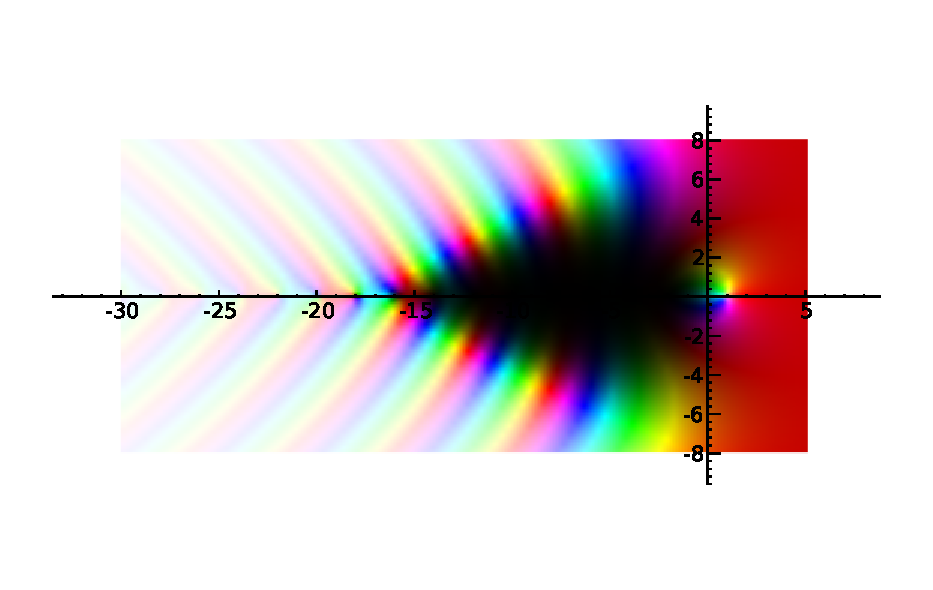
\includegraphics[width=15em]{zeta.eps}

$\displaystyle \zeta(s) = \prod_{p} \frac{1}{1-p^{-s}} = \sum \frac{1}{n^s} = $ \EX{zeta(s)}

$\displaystyle \operatorname{Li}(x) = \int_{2}^{x} \frac{1}{\log(t)} dt = $ \EX{Li(x)}

$\displaystyle \Gamma(s) = \int_0^{\infty} t^{s-1}e^{-t}dt = $ \EX{gamma(s)}


\vspace{6ex}
\makebox{}

%*********************************************
\sect{Continued Fractions}

{\tiny \sagecommand{continued_fraction(pi)}}
{\small $$
\pi = 3+ \frac{\displaystyle 1}{\displaystyle 7+ \frac{\displaystyle 1}{\displaystyle 15+ \frac{\displaystyle 1}{\displaystyle 1+ \frac{\displaystyle 1}{\displaystyle 292 + \cdots}}}}$$}

continued fraction: \EX{c=continued_fraction(x,}\EXVAR{bits}\EX{)}

convergents: \EX{c.convergents()}

convergent numerator $p_n =$ \EX{c.pn(n)}

convergent denominator $q_n =$ \EX{c.qn(n)}

value: \EX{c.value()}

 
%*********************************************
\sect{Elliptic Curves}

{\tiny\sagecommand{EllipticCurve([0,0,1,-1,0]).plot(plot_points=300,thickness=3)}}
\BreakLineAndIndent
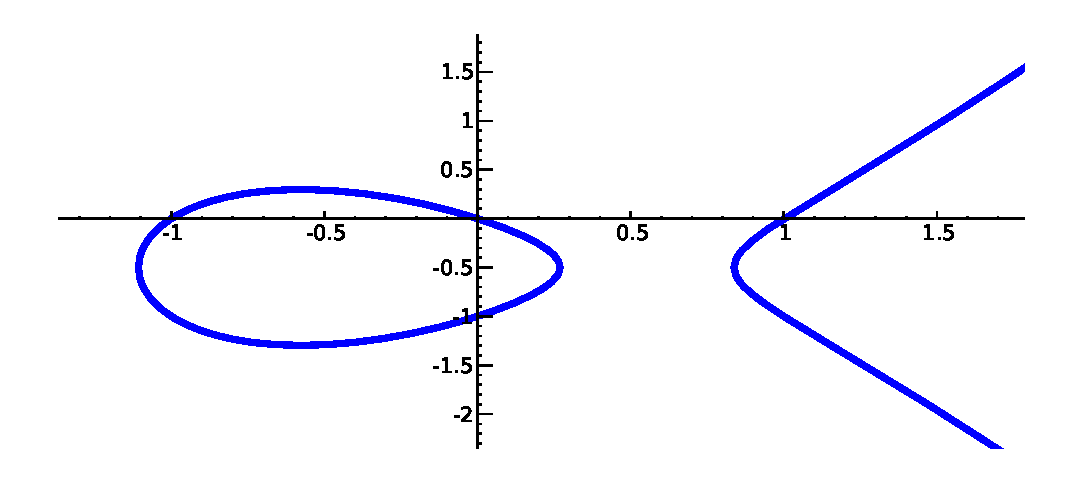
\includegraphics[width=10em]{ec.eps}

\mbox{}\quad\EX{E = EllipticCurve([}$a_1,a_2,a_3,a_4,a_6$\EX{])}
\vspace{-1ex}
$$y^2 + a_1 xy + a_3 y = x^3 + a_2 x^2 + a_4 x + a_6$$

conductor $N$ of $E = $\EX{E.conductor()}

discriminant $\Delta$ of $E = $\EX{E.discriminant()}

rank of $E =$  \EX{E.rank()}

free generators for $E(\QQ) = $ \EX{E.gens()}

$j$-invariant $=$ \EX{E.j_invariant()}

$N_p = \#\{\text{solutions to $E$ modulo $p$}\} = $ \EX{E.Np(}\EXVAR{prime}\EX{)}

$a_p = p+1 - N_p = $\EX{E.ap(}\EXVAR{prime}\EX{)}

$L(E,s) = \sum \frac{a_n}{n^s} = $ \EX{E.lseries()}

$\operatorname{ord}_{s=1}L(E,s) = $ \EX{E.analytic_rank()}


%*********************************************
\sect{Elliptic Curves Modulo $p$}

{\tiny\sagecommand{EllipticCurve(GF(997), [0,0,1,-1,0]).plot()}}

\mbox{}\qquad\qquad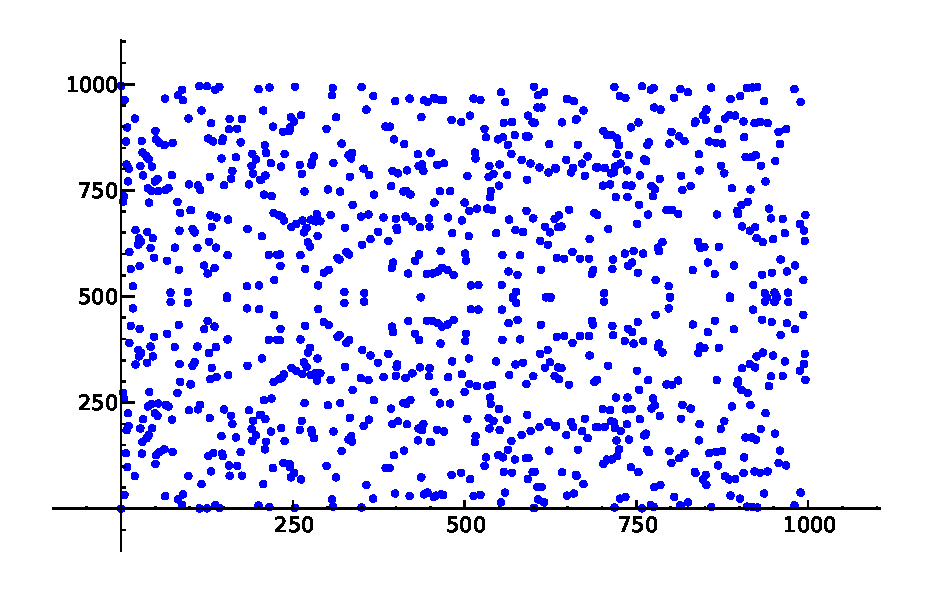
\includegraphics[width=7em]{ecmodp.eps}

\mbox{}\quad\EX{E = EllipticCurve(GF(p), [}$a_1,a_2,a_3,a_4,a_6$\EX{])}

$\#E(\FF_p) = $ \EX{E.cardinality()}

generators for $E(\FF_p) = $ \EX{E.gens()}

$E(\FF_p) = $\EX{E.points()}










%%*********************************************
% \hr\textbf{Binary Quadratic Forms}
%\texttt{QuadraticForm}

%*********************************************
% \hr\textbf{Quadratic Fields}
%\texttt{ZZ[I]}
%\texttt{QuadraticField}

%*********************************************
% \hr\textbf{Cyclotomic Fields}
%\texttt{CyclotomicField}
%\texttt{Gauss sums}


%*********************************************
% \hr\textbf{Finite Fields}
%\texttt{GF(q)}



\end{multicols*}

\end{document}
